\documentclass[a4paper,12pt]{report}

\usepackage{cmap}
\usepackage[T2A]{fontenc}
\usepackage[utf8]{inputenc}
\usepackage[english,russian]{babel}
\usepackage{listings}
\usepackage{amsmath}
\usepackage{float}
\usepackage{csquotes}
\usepackage{mathtools}
\usepackage{hyphenat}
\usepackage{amsfonts}
\usepackage{upgreek}

\usepackage{xcolor}
\usepackage{hyperref}

\usepackage{graphicx}
\graphicspath{ {./img/} }

\definecolor{dkgreen}{rgb}{0,0.6,0}
\definecolor{gray}{rgb}{0.5,0.5,0.5}
\definecolor{mauve}{rgb}{0.58,0,0.82}

\lstset{
    language=Python,                 % выбор языка для подсветки (здесь это С)
    basicstyle=\small\sffamily, % размер и начертание шрифта для подсветки кода
    numbers=left,               % где поставить нумерацию строк (слева\справа)
    numberstyle=\tiny,           % размер шрифта для номеров строк
    stepnumber=1,                   % размер шага между двумя номерами строк
    numbersep=5pt,                % как далеко отстоят номера строк от подсвечиваемого кода
    aboveskip=3mm,
    belowskip=3mm,
    showstringspaces=false,
    columns=flexible,
    captionpos=b, 
    basicstyle={\small\ttfamily},
    numbers=left,
    numberstyle=\tiny\color{gray},
    keywordstyle=\color{blue},
    commentstyle=\color{mauve},
    stringstyle=\color{dkgreen},
    breaklines=true,
    breakatwhitespace=true,
    tabsize=3
}

\title{Лабораторная работа №10\\Линейные стационарные системы}
\author{Смирнов Никита}
\date{\today}

\begin{document}

\maketitle
\tableofcontents
\listoffigures
\lstlistoflistings

\maketitle

\chapter{Упражнение 10.1}

Усечём сигналы до $2^{16}$ значений, а затем обнудим их до $2^{17}$.

Я взял запись выстрела и сделал над ним изменения.

\begin{lstlisting}[caption=Усечение сигнала]
response = thinkdsp.read_wave('180960__kleeb__gunshot.wav')

start = 0.12
response = response.segment(start=start)
response.shift(-start)

response.truncate(2**16)
response.zero_pad(2**17)

response.normalize()
response.plot()
thinkplot.config(xlabel='Time (s)', ylim=[-1.05, 1.05])
\end{lstlisting}

Получил следующее изображение:

\begin{figure}[H]
        \centering
        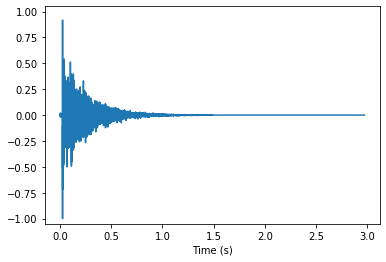
\includegraphics[width=0.75\textwidth]{1.png}
        \caption{Визуализация сигнала}
        \label{1}
\end{figure}

Вычисляю спектр:

\begin{lstlisting}[caption=Спектр сигнала]
transfer = response.make_spectrum()
transfer.plot()
thinkplot.config(xlabel='Frequency (Hz)', ylabel='Amplitude')
\end{lstlisting}

\begin{figure}[H]
        \centering
        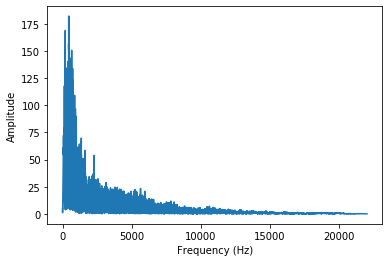
\includegraphics[width=0.75\textwidth]{2.png}
        \caption{Спектр сигнала}
        \label{2}
\end{figure}

Создаю другой сигнал:

\begin{lstlisting}[caption=Усечение сигнала]
violin = thinkdsp.read_wave('92002__jcveliz__violin-origional.wav')

start = 0.11
violin = violin.segment(start=start)
violin.shift(-start)

violin.truncate(2**16)
violin.zero_pad(2**17)

violin.normalize()
violin.plot()
thinkplot.config(xlabel='Time (s)', ylim=[-1.05, 1.05])
\end{lstlisting}

\begin{figure}[H]
        \centering
        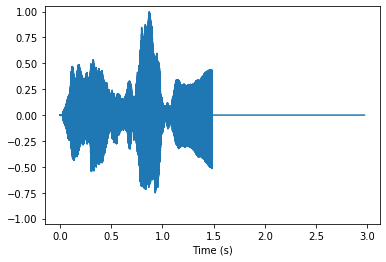
\includegraphics[width=0.75\textwidth]{3.png}
        \caption{Визуализация сигнала}
        \label{3}
\end{figure}

Составим спектр:

\begin{lstlisting}[caption=Спектр сигнала]
spectrum = violin.make_spectrum()
\end{lstlisting}

Теперь умножим ДПФ сигнала на передаточную функцию и преобразуем обратно в волну:

\begin{lstlisting}[caption=Совмещение сигнала]
output = (spectrum * transfer).make_wave()
output.normalize()
output.plot()
\end{lstlisting}

\begin{figure}[H]
        \centering
        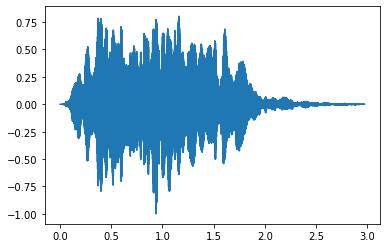
\includegraphics[width=0.75\textwidth]{4.png}
        \caption{Визуализация сигнала}
        \label{4}
\end{figure}

Лишнюю ноту в начале не слышно. Избавимся от нулевого отступа:

\begin{lstlisting}[caption=Избавление от нулевого отступа]
response.truncate(2**16)
response.plot()

violin.truncate(2**16)
violin.plot()
\end{lstlisting}

\begin{figure}[H]
        \centering
        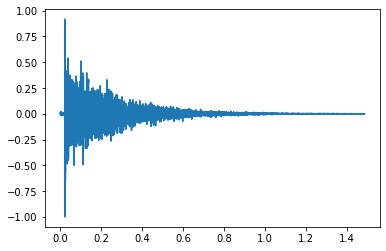
\includegraphics[width=0.75\textwidth]{5.png}
        \caption{Визуализация сигнала}
        \label{5}
\end{figure}

\begin{figure}[H]
        \centering
        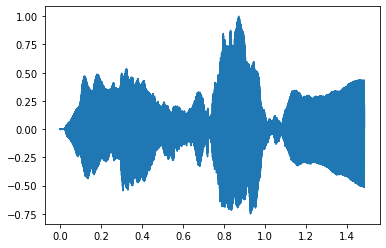
\includegraphics[width=0.75\textwidth]{6.png}
        \caption{Визуализация сигнала}
        \label{6}
\end{figure}

Теперь мы можем сравнить с \texttt{np.convolve}:

\begin{lstlisting}[caption=Объединение сигналов]
output2 = violin.convolve(response)
output2.plot()
\end{lstlisting}

\begin{figure}[H]
        \centering
        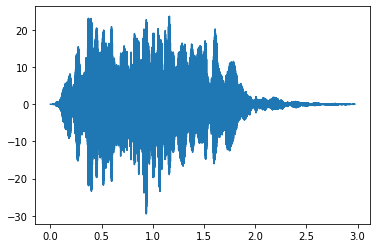
\includegraphics[width=0.75\textwidth]{7.png}
        \caption{Визуализация сигнала}
        \label{7}
\end{figure}

Результаты похожи. Звук такой же, но длина не та.

\begin{lstlisting}[caption=Сравнение длин сигналов]
len(output), len(output2)
\end{lstlisting}

На выходе получились значения \texttt{(131072, 131071)}.

\texttt{scipy.signal.fftconvolve} делает то же самое, но, как следует из названия, он использует ДПФ, поэтому он значительно быстрее:

\begin{lstlisting}[caption=Изменение сигнала]
import scipy.signal
ys = scipy.signal.fftconvolve(violin.ys, response.ys)
output3 = thinkdsp.Wave(ys, framerate=violin.framerate)
\end{lstlisting}

\begin{lstlisting}[caption=Визуализация сигнала]
output3.plot()
\end{lstlisting}

\begin{figure}[H]
        \centering
        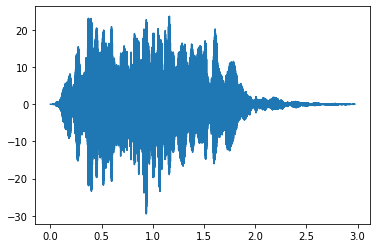
\includegraphics[width=0.75\textwidth]{8.png}
        \caption{Визуализация сигнала}
        \label{8}
\end{figure}

Результат тот же. В пределах ошибки с плавающей запятой результаты такие же:

\begin{lstlisting}[caption=Сравнение результатов]
output2.max_diff(output3)
\end{lstlisting}

Ошибка равна \texttt{2.1316282072803006e-14}.

\chapter{Упражнение 10.2}

Для начала я взял запись, которая будет использована в качестве испульсной характеристики.

\begin{lstlisting}[caption=Загрузка звука]
response = thinkdsp.read_wave('mono.wav')

start = 0
duration = 5
response = response.segment(duration=duration)
response.shift(-start)

response.normalize()
response.plot()
thinkplot.config(xlabel='Time (s)', ylim=[-1.05, 1.05])
\end{lstlisting}

\begin{figure}[H]
        \centering
        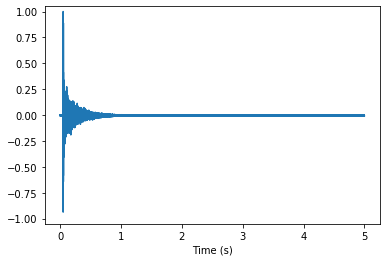
\includegraphics[width=0.75\textwidth]{9.png}
        \caption{Визуализация звука}
        \label{9}
\end{figure}


\begin{lstlisting}[caption=Спектр звука]
transfer = response.make_spectrum()
transfer.plot()
thinkplot.config(xlabel='Frequency (Hz)', ylabel='Amplitude')
\end{lstlisting}

\begin{figure}[H]
        \centering
        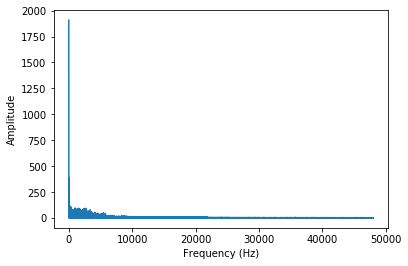
\includegraphics[width=0.75\textwidth]{10.png}
        \caption{Спектр звука}
        \label{10}
\end{figure}

Рассмотрим передаточную функцию:

\begin{lstlisting}[caption=Визуализация звука]
transfer.plot()
thinkplot.config(xlabel='Frequency (Hz)', ylabel='Amplitude',
                 xscale='log', yscale='log')
\end{lstlisting}

\begin{figure}[H]
        \centering
        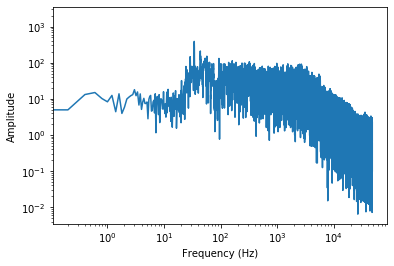
\includegraphics[width=0.75\textwidth]{11.png}
        \caption{Визуализация звука}
        \label{11}
\end{figure}

Беру вторую запись с такой же частатой дескритизации:

\begin{lstlisting}[caption=Загрузка звука]
wave = thinkdsp.read_wave('38849.wav')

start = 0.0
wave = wave.segment(start=start)
wave.shift(-start)

wave.truncate(len(response))
wave.normalize()
wave.plot()
thinkplot.config(xlabel='Time (s)', ylim=[-1.05, 1.05])
\end{lstlisting}

\begin{figure}[H]
        \centering
        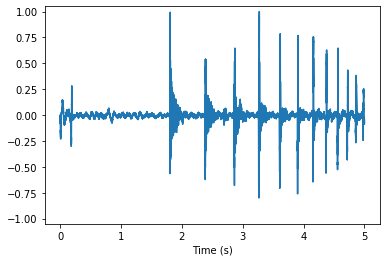
\includegraphics[width=0.75\textwidth]{12.png}
        \caption{Визуализация звука}
        \label{12}
\end{figure}

Смотрим частоту дискретизации.

\begin{lstlisting}[caption=Частота дискретизации 1]
from pydub import AudioSegment
song = AudioSegment.from_mp3("mono.wav")
song.frame_rate
\end{lstlisting}

\begin{lstlisting}[caption=Частота дискретизации 2]
song2 = AudioSegment.from_mp3("38849.wav")
song2.frame_rate
\end{lstlisting}

Оба звука имеют частоту дискретизации 96000.

Теперь мы вычисляем ДПФ.

\begin{lstlisting}[caption=Спектр звука]
spectrum = wave.make_spectrum()
\end{lstlisting}

Обрежем запись до той же длины, что и импульсная характеристика:

\begin{lstlisting}[caption=Длина записей]
len(spectrum.hs), len(transfer.hs)
\end{lstlisting}

Длины совпадают и равны \texttt{(240001, 240001)}.

\begin{lstlisting}[caption=Длина первой записи]
spectrum.fs
\end{lstlisting}

\begin{lstlisting}[caption=Длина второй записи]
transfer.fs
\end{lstlisting}

Массивы значений совпадают и равны \texttt{array([    0. ,     0.2,     0.4, ..., 47999.6, 47999.8, 48000. ])}.

Мы можем умножить в частотной области и преобразовать обратно во временную область.

\begin{lstlisting}[caption=Перемножение]
output = (spectrum * transfer).make_wave()
output.normalize()
\end{lstlisting}

Рассмотрим сравнение оригинальной и преобразованной записи:

\begin{lstlisting}[caption=Визуализация оригинального звука]
wave.plot()
\end{lstlisting}

\begin{figure}[H]
        \centering
        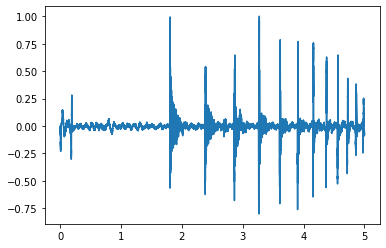
\includegraphics[width=0.75\textwidth]{13.png}
        \caption{Визуализация оригинального звука}
        \label{13}
\end{figure}

\begin{lstlisting}[caption=Визуализация преображённого звука]
output.plot()
\end{lstlisting}

\begin{figure}[H]
        \centering
        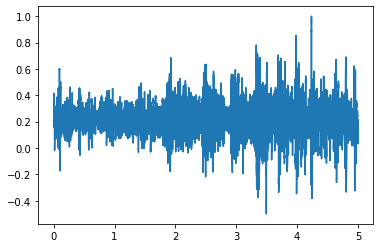
\includegraphics[width=0.75\textwidth]{14.png}
        \caption{Визуализация преображённого звука}
        \label{14}
\end{figure}

Теперь, когда мы распознаем эту операцию как свёртку, мы можем вычислить ее с помощью метода \texttt{convolve}:

\begin{lstlisting}[caption=Моделирование при помощи \texttt{convolve}]
convolved2 = wave.convolve(response)
convolved2.normalize()
convolved2.make_audio()
\end{lstlisting}

\chapter{Выводы}

Во время выполнения лабораторной работы получены навыки работы с теорией сигналов и систем, а также применения теоремы свёртки, характеризуя линейные, инвариантные во времени системы.

\end{document}